
        \chapter{Sortieren}
        Warum?
        \begin{itemize}
            \item viele Konzepte des Algorithmen-Design und -Vergleichs werden sehr anschaulich
            \item sortierte Daten braucht man oft in der Praxis, z.B. zum schnellen Suchen
            \item aber: man muss sortieren heute selten selbst implementieren, weil alle Programmiersprachen das schon anbieten \\
            \hspace*{1cm} \verb|sort(a)|
        \end{itemize}

        \textbf{Spielregeln}:
        \begin{enumerate}
            \item Die Daten liegen in einem Array: \verb|a| \\
            $\Rightarrow$ Der Alg. darf aufrufen: \\
        \end{enumerate}
        \vspace*{-5mm}
        \begin{minted}{python}
            N = len(a)              # Laenge von a
            v = a[i]                # Lesen von El.i
            a[i] = v                # Schreiben von El.i
        \end{minted}

        mit $i \in [0, N-1]$ \\
        $\Rightarrow$ Der zu sortierende Datentyp ($\widehat{=}$ Elemente des Arrays) unterstützen in Vergleichsfunktion, meist ``$<$'' \\
        $a[i] < a[k] \Rightarrow$ \verb|True oder False| \\

        Der Vergleich muss die mathematischen Anforderungen einer \emph{totalen Ordnung} erfüllen \\


        Eine totale Ordnung ist antisymmetrisch, transitiv, reflexiv, total \\
        Elemente $a,b,c,...$ und die Relation ``$\leq$'': $a \leq b \rightarrow$ \verb|t, f| \\
        \begin{itemize}
                \item total: man kann beliebige Elementpaare vergleichen \\
                $a \leq b$ liefert immer \verb|t oder f| \\
                (Gegenteil: Halbordnung: manche Elemente nicht vergleichbar
                $a\leq b$ liefert \verb|t oder f oder "unknown"|)

                \item antisymmetrisch: $a \leq b \land b \leq a \Rightarrow a == b$
                \item transitiv: $ a \leq b \land b \leq c \Rightarrow a \leq c$
                \item reflexiv: (folgt aus den anderen): $a \leq a$ immer \verb|true|
        \end{itemize}

            Frage: Angenommen $a \leq b$ ist definiert, aber der Sortieralgorithmus braucht $a < b$. \\
            Kann man $a < b$ implementieren, indem man nur logische Operationen $\land \lor \lnot$ sowie $\leq$ verwendet? \\

            Antwort: $a < b \Leftrightarrow \lnot(b \leq a)$ \\

            Hausaufgabe: Wie bekommt man $>, \geq, ==, !=$ \\

            \section{Selection Sort}

            \begin{minted}{python}
def selection_sort(a):
    N = len(a)
    for i in range(N-1):        # i ist die Arrayposition, die wir sortieren wollen
        m = i                   # m ist unsere aktuelle Meinung,
                                # wo das kleinste rechts von i steht
        for k in range(i+1, N):
            if a[k] < a[m]:
                m = k           # Meinung korrigieren
                                # a[m] ist jetzt das kleinste Element rechts von i
        a[i], a[m] = a[m], a[i] # vertauschen
            \end{minted}
            \begin{itemize}
                \item Datenobjekte haben oft mehrere Eigenschaften, nach denen man sortieren kann. \\
                Studenten: Sortieren nach Alter, Alda-Noten, ... \\
                hier: nach Zahl oder Farbe\\
                sortiere jetzt nach Farbe: orange $<$ rot$ <$ blau $<$ schwarz

                \textbf{Stabiliät der Sortierung}:
                \begin{itemize}
                    \item Anfangs ist das Array nach Kriterium 1 sortiert (``Zahl'')
                    \item Wir sortieren nun nach Kriterium 2 (``Farbe''), aber es gibt Elemente, die dabei den gleichen Wert haben
                    \item Sortieralgorithmus ist \emph{stabil}, wenn die Ordnung 1 erhalten bleibt, über Elementen mit identischem Wert 2
                \end{itemize}
            \end{itemize}
            $\Rightarrow$ Selection Sort nicht stabil \\

            \section{Insertion Sort}
            ähnlich einfach wie Selection Sort, aber \emph{stabil}
            \begin{itemize}
                \item Beobachtung: Insertion Sort ist für \emph{kleine Arrays} (N $<$ 30) der schnellste Sortieralgorithmus \\
            \end{itemize}
            \begin{minted}{python}
def insertion_sort(a):
    N = len(a)
    for i in range(N):
        current = a[i]
        k = i
        while k > 0:
            if current < a[k - 1]:
                a[k] = a[k - 1]
            else:
                break
            k = k - 1
    a[k] = current
            \end{minted}

            Welche Laufzeit benötigen Selection und Insertion Sort?
            \begin{itemize}
                \item Wie misst man das unabhängig davon, ob man einen schnellen oder langsamen Computer hat, oder wie groß N ist?
                \item 2 Lösungen: Zähle a Anzahl der Vergleiche $a < b$, b Anzahl der Vertauschungen \\
            \end{itemize}

        \begin{tabular}{C{3cm} | R{5cm}}
                i & Anzahl der Schritte in der Schleife $\widehat{=}$ Anzahl Vergleiche \\ \hline
                0 & $k \in [1, N-1] \widehat{=} N-1$ S. \\
                1 & $[2, N-1] \widehat{=} N-2$ S. \\
                2 & $\widehat{=} N-3$ S. \\
                $\vdots$ & \\
                $N-2$ & $[N-1, N-1] \widehat{=} 1$ S. \\
        \end{tabular}

    $\Rightarrow$ die totale Anzahl Vergleiche: \\
    $T = (N-1)+(N-2)+(N-3)+...+2+1$\\

    \fbox{$= \frac{N(N-1)}{2} \approx \frac{N^2}{2}$}\\

    Anzahl Vertauschungen: $ V = N-1 < T$


    \subsection*{Elementare Sortierverfahren}
    iteriere mit i über alle Arrayelemente

    \begin{itemize}
        \item Selection Sort: finde das $\underline{\text{kleinste}}$ Element $\underline{\text{rechts}}$ von i und bringe es auf Position i
        \item Insertion Sort: Finde die passende $\underline{\text{Lücke}}$ $\underline{\text{links}}$ von i, wo Element a[i] einsortiert werden muss

    \end{itemize}

    \subsection{Aufwand beim Sortieren}
    Aufwand beim Sortieren: Anzahl der Vergleiche $a[i] < a[k]$ und/oder Anzahl der Vertauschungen $a[i],a[k] = a[k], a[i]$

    \begin{itemize}
        \item bei Selection Sort: Anzahl Vergleiche $V = \frac{N(N-1)}{2}$
        \item bei Insertion Sort: Unterscheide drei Fälle:
        \begin{itemize}
            \item günstigster Fall: Array schon sortiert
            \item ungünstigster Fall: Array umgekehrt sortiert (absteigend statt aufsteigend)
            \item typischer Fall: Array zufällig angeordnet
        \end{itemize}
        \item alle drei Fälle haben unterschiedliches V! \\
        (bei Selection Sort: V immer gleich)

    \end{itemize}

    \begin{minted}{python}
def insertion_sort_1(a):
    N = len(a)
    for i in range(1, N):
        k = i
        while k > 0:
            if a[k] < a[k - 1]:
                a[k - 1], a[k] = a[k], a[k - 1]
            else:
                break
            k = k - 1
    \end{minted}

    $\Rightarrow$ für kleine N der schnellste Algorithmus \\
    \vspace*{-5mm}
    \begin{enumerate}
        \item günstigster Fall: Array ist sortiert, d.h. der Vergleich (*) liefert immer sofort ``False" '$\Rightarrow$ while-Schleife hat nur 1 Iteration \\
        $\Rightarrow$ ein Vergleich pro i $\Rightarrow$\fbox{$V = N-1$}
        \item ungünstigster Fall: Array umgekehrt sortiert $\Rightarrow$ Vergleich (*) liefert immer ``True'' $\Rightarrow$ while-Schleife muss immer bis zum Ende (k=0) durchlaufen werden $\Rightarrow$ i Vergleiche für jedes i \\
        $V=1+2+3+...+(N-1)=$ \fbox{$\frac{N(N-1)}{2} = V$} $\approx$ \fbox{$\frac{N^2}{2}$}
        \item typischer Fall: Array zufällig $\Rightarrow$ im $\underline{\text{Mittel}}$ wird die while-Schleife zur Hälfte durchlaufen $\Rightarrow$ \fbox{$V = \frac{N(N-1)}{4}$} $\approx$ \fbox{$\frac{N^2}{4}$}
    \end{enumerate}


    Einwurf: \\
    swap braucht mindestens 3 Zuweisungen: \\
    \hspace*{5mm} swap(a,b) : tmp = a, a = b, b = tmp \\
    in Python: sogar 4 a,b = b,a $\widehat{=}$ t1=a, t2=b, b=t1, a=t2


    \subsection*{Sortieren nach dem Teile-und-Herrsche-Prinzip}

    \begin{itemize}
        \item elementare Alg. brauchen im typischen Fall $V= c * N^2$ Vergleiche für eine Konstante c $\Rightarrow$ sie sind für große N langsam
        \item bessere Alg.: teilen das Sortierproblem in Unterprobleme, die getrennt sortiert und dann effizient zusammengesetzt werden.

    \end{itemize}

    \section{Merge Sort}

    \begin{itemize}
        \item Operation merge: Setze ein großes Array aus zwei sortierten Teilarrays zusammengesetzt
    \end{itemize}

    \begin{minted}{python}
def merge(l, v):  # l,r: sortierte Teilarrays
    a = []  # leeres Array fuer das Ergebnis
    i, k = 0, 0
    Nl, Nr = len(l), len(r)
    while i < Nl and k < Nr:
        if l[i] <= r[k]:
            a.append(l[i])
            i = i + 1
        else:
            a.append(r[k])
            k = k + 1

    a = a + l[i:Nl] + r[k:Nr]  # Rest von l bzw. r an a anhaengen
    return a
    \end{minted}


    \verb|r[k : Nr]| entspricht: \\
    \begin{minted}{python}
    while k < Nr:
        n.append(r[k])
        k = k+1
    while i < Nl:
        n.append(l[i])
        i = i+1
    \end{minted}


    \begin{itemize}
        \item um l und r zu sortieren, wendet man das gleiche Prinzip $\underline{\text{rekursiv}}$ auf die linke bzw. rechte Hälfte des Arrays an:
    \end{itemize}

    \begin{minted}{python}
def merge_sort(a):
    N = len(a)
    if N <= 1:                            # leeres Array oder mit 1 Element
        return a                          # ist automatisch sortiert
    else:
        l = a[0:N//2]                     # N//2 = "floor division", rundet ab
        r = a[N//2 : N]
        l_sorted = merge_sort(l)          # teile-und-herrsche
        r_sorted = merge_sort(r)
        a_sorted = merge(l_sorted, r_sorted)
        return a_sorted
    \end{minted}

        \textbf{Laufzeit von merge sort:} \\
        \begin{itemize}
            \item Wie tief ist der Baum, der bei der Ausführung entsteht?
        \end{itemize}

        Beispiel für $N=8$


        \begin{center}
            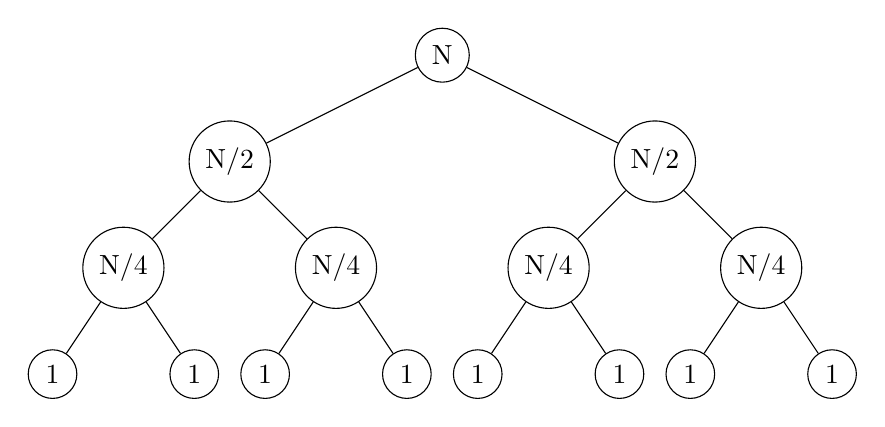
\begin{tikzpicture}[scale=0.9,level/.style={sibling distance=60mm/#1}]
            \node[circle, draw] (a) {N}
            child {node [circle, draw] (b) {N/2}
                child {node [circle, draw] (c) {N/4}
                    child {node [circle, draw] (d) {1}}
                    child{node [circle, draw] (e) {1}}}
                child {node [circle, draw] (f) {N/4}
                    child {node [circle, draw] (g) {1}}
                    child {node [circle, draw] (h) {1}}}
            }
            child {node [circle, draw] (i) {N/2}
                child {node [circle, draw] (j) {N/4}
                    child {node [circle, draw] (k) {1}}
                    child {node [circle, draw] (l) {1}}}
                child {node [circle, draw] (m) {N/4}
                    child {node [circle, draw] (n) {1}}
                    child {node [circle, draw] (o) {1}}}
            };
            \end{tikzpicture}
        \end{center}

        $8 = 2^3 \Rightarrow$: \fbox{$M + 1 = \text{Tiefe} = \ceil{log_2 N}$} \\

        Wie viele Vergleiche braucht man pro Ebene? \\

        \hspace*{5mm} $\rightarrow$ Ebene 1: Zwei Arrays der Länge N/2 \\
        \hspace*{7mm} $\Rightarrow$ merge vergleicht immer die ersten Elemente von l und r \\
        \hspace*{5mm} ungünstigster Fall: das kleinste Element ist abwechselnd links und rechts $\Rightarrow$ (N-1) Vergleiche $\approx$ N Vergleiche \\

        dazu kommen die Vergleiche für das Sortieren der Teilarrays l und r \\

        \hspace*{5mm} $ \Rightarrow  V(N)= \underbrace{N}_{\approx N-1} + \underbrace{2}_{\text{2 Arrays}}* \underbrace{(N/2)}_{\text{der Länge N/2 sortieren}} $ \\

        \hspace*{19.5mm} $= N + \underbrace{[\frac{N}{2} + 2 * V(\frac{N}{4})]}_{\text{l sortieren}} + \underbrace{[\frac{N}{2} + 2 * V(\frac{N}{4})]}_{\text{r sortieren}}$ \\

        \hspace*{19.5mm} $= N + (\frac{N}{2} + \frac{N}{2}) + 4 * [\frac{N}{4} + 2 * V(\frac{N}{8})] $\\

        \hspace*{19.5mm} $= N + \underbrace{(\frac{N}{2} + \frac{N}{2})}_{N} + \underbrace{4 * (\frac{N}{4}}_{N}) + \cdots $\\

        \hspace*{19.5mm} $= N + N + N + \cdots + N$

        \begin{itemize}[label={$\Rightarrow$}]
            \item pro Zerlegungsebene N Vergleiche (bzw. Zuweisungen)
            \item da es $\ceil{log_2 N}$ Ebenen gibt, ist die Gesamtzahl der Vergleiche
        \end{itemize}

        \hspace*{5mm} \fbox{$V = N * \ceil{log_2 N}$} $<< \frac{N^2}{4}$ für große N \\


        günstiger Fall: Array bereits sortiert \\

        $\Rightarrow$ bei merge werden zuerst alle Elemente von l gewählt, dann r an das Ergebnis-Array angehängt \\

        $\Rightarrow$ man braucht nur halb so viele Vergleiche wie im ungünstigen Fall \\

        \hspace*{5mm} $V= \frac{N}{2} \ceil{log_2(N)} = c N * \ceil{log_2(N)}$ \\

        unterscheidet sich nur durch Konstante c $\widehat{=}$ unwichtig \\

        \begin{itemize}
            \item Merge Sort ist $\underline{\text{stabil}}$, wenn bei Gleichheit l[i] == r[k] immer das $\underline{\text{linke}}$ Element gewählt wird
            \item Python's list.sort()-Funktion verwendet merge sort wegen der Stabilität\\
            $\underline{\text{aber}}$: hochoptimiert, d.h. häufige Spezialfälle (bereits sortiert, umgekehrt sortiert) werden abgefangen und schneller implementiert
        \end{itemize}

    \section{Quick Sort}

    \begin{itemize}
        \item Standard-Algorithmus für Sortieren, z.B. in vielen Implementationen von C++:  std::sort() \\
        (optimierte Kombination von Quick Sort mit heap sort \& insertion sort)
        \item Nachteil von merge sort: es braucht temporären Speicher zum Anlegen der gemergten Arrays
        \item besser: in-place $\widehat{=}$ sortieren erfolgt im Originalarray \\
        $\Rightarrow$ quick sort
        \item Idee: Funktion ``partition'': wähle Pivot-Element und sortiere es an die korrekte Stelle $\Rightarrow$ alle linken sind kleiner, alle rechten größer, aber nicht untereinander sortiert
    \end{itemize}

    \begin{minted}{python}
def partition(a, l, r):       # l: linke Grenze des zu sortierenden Bereichs
    pivot = a[r]              # r: rechte Grenze
    i = l, k = r - 1
    while True:               # Endlosschleife -> wird unten per "break" verlassen
        while i < r and a[i] <= pivot: # suche Element > pivot
            i = i+1
        while k > l and a[k] >= pivot: # suche Element < pivot
            k = k - 1
        if i < k :
            a[i], a[k] = a[k}, a[i]    # tausche oder beende Schleife
        else:
            break
    a[r] = a[i]
    a[i] = pivot              # bringe pivot an richtige Pos.
    return i                  # pivot-Position fuer Rekursion

def quick_sort(a):
    quick_sort_impl(a, 0, len(a)-1)
    (return a)

def quick_sort_impl(a, l, r):
    if r <= l :            # a[l : r + 1] hat hoechstens ein Element -> schon sortiert
        return (None)
    k = partition(a, l, r) # k ist korrekte Position des Pivot
    quick_sort_impl(a, l, k-1)  # rekursiv links
    quick_sort_impl(a, k+1, r)  # rekursiv rechts
    \end{minted}

    \subsection*{Laufzeit von Quick Sort}
    \begin{itemize}
        \item günstiger Fall: das Pivot ist bei jedem Aufruf immer der Median des Teilarrays ($\widehat{=}$ Element in der Mitte, nach partition())\\
        $\Rightarrow$ die verbleibenden Teilarrays sind ungefäht gleichgroß \\

        Rekursionsformel: allg. Prinzip: $\underbrace{C(N)}_{\text{totale Laufzeit für Größe N}} = \underbrace{A(N)}_{\text{Laufzeit im aktuellen Teilarray}} + \underbrace{R(N)}_{\text{Laufzeit für rekursive Aufrufe}}$\\

        \verb|C(quick_sort_imp(N)) = C(partition(N)) + C(qsi(links)) + C(qsi(rechts))| \\

        \vspace*{-5mm}
        $C_g(N) \approx (N+1)+C_g(\frac{N}{2} -1) + C_g(\frac{N}{2} -1)$\\

        \vspace*{-5mm}
        $\approx N + 2+ C_g(\frac{N}{2}) = N*\ceil{log_2(N)}$

        \item ungünstiger Fall: Pivot ist immer am Rand, d.h. partition() verändert die Position des Pivots nicht $\widehat{=}$ Array war schon sortiert \\
        $C_u(N) = \underbrace{(N+1)}_{\text{partition}} + \underbrace{C_u(N - 1) + C_u(0)}_{\text{Rekursion}} \hspace*{1cm} C_u(0)=0$ \\

        \vspace*{-5mm}
        $ = (N+1) + [N + C_u(N-2)]$ \\

        \vspace*{-5mm}
        $= (N+1) + N + \biggl\lbrack(N-1) + C_u(N-3)\biggr\rbrack$ \\

        \vspace*{-5mm}
        $ = (N+1) + N + ... + 1 = \frac{(n+2)(N+1)}{2} \approx \frac{N^2}{2}$ \\
        \vspace*{-2mm}
        $\Rightarrow$ so langsam wie selection sort $\Rightarrow$ wir müssen den ungünstigen Fall verhindern

        \item typischer Fall: Array ist zufällig sortiert \\
        $\Rightarrow$ jede Position zwischen l und r ist mit gleicher Wahrscheinlichkeit die Position des Pivot nach partition() \\
        $\Rightarrow$ wir verwenden den Mittelwert des Aufwands in der Rekursionsformel \\
        \[C_t(N) = (N+1) + \frac{1}{N}  \hspace*{-9mm} \underbrace{\underbrace{\sum_{k=1}^N}_{\text{mögliche Pos. des Pivots}}\hspace*{-9mm} [C_t(k-1) + C_t(N-k)]}_{= 2 \sum_{k=1}^N C_t(k-1)} \]\\
        \vspace*{-6mm}
        \[N * C_t(N) = (N+1) * N + 2 \sum_{k=1}^N C_t(k-1)\] \\
        \vspace*{-6mm}
        \[ \begin{rcases}(N-1) C_t(N-1) = N*(N-1) + 2 & \\
         N * C_t(N) = (N+1) * N + 2 \sum_{k=1}^{N-1} C_t(k-1) & \end{rcases} - \]\\
         \vspace*{-6mm}
        \[N* C_t(N) - (N-1) C_t(N-1) = (N+1)N - N(N-1) + 2 C_t(N-1) \] \\
        \vspace*{-9mm}
        \[ N * C_t(N) = (N+1) * C_t(N-1) + 2N \hspace*{4mm} \big| :N\] \\
        \vspace*{-9mm}
        \[ C_t(N) = \frac{N+1}{N} C_t(N-1) + 2* \frac{N+1}{N+1} \] \\
        \vspace*{-9mm}
        \[ (N+1) \biggl\lbrack \frac{1}{N} C_t(N-1) + \frac{2}{N+1}\biggr\rbrack \] \\
        $ C_t(N-1)$ sukzessive expandieren \\
        \vspace*{-3mm}
        \[ C_t(N) = (N+1) \hspace*{1mm}  \biggl\lbrack \frac{1}{\slashed{N}} \frac{\slashed{N}}{N-1} C_t(N-2) + 2 \frac{N}{N} + \frac{2}{N+1}\biggr\rbrack\] \\
        \vspace*{-9mm}
        \[ = \frac{N+1}{N-1} \hspace*{1mm} C_t(N-2) + 2(N+1) \hspace*{1mm} \biggl\lbrack\frac{1}{N}+\frac{1}{N+1}\biggr\rbrack \]\\
        \vspace*{-9mm}
        \[ = \frac{N+1}{N-2} \hspace*{1mm} C_t(N-3) + 2(N+1)  \hspace*{1mm}\biggl\lbrack\frac{1}{N}+\frac{1}{N+1}+ \frac{1}{N+1}\biggr\rbrack\] \\
        \vspace*{-9mm}
        \[= \frac{N+1}{1} \hspace*{1mm} \underbrace{C_t(0)}_{=0} + 2(N+1)  \hspace*{1mm} \underbrace{\biggl\lbrack \frac{1}{3} + \frac{1}{4} + \dots + \frac{1}{N+1}\biggr\rbrack}_{< \frac{1}{1}+ \frac{1}{2}+ \frac{1}{3}+\frac{1}{4}+\dots+\frac{1}{N+1}} \]\\
        \vspace*{-7mm}
        \[\leq 2(N+1)\hspace*{-7mm}\underbrace{ \sum_{k=1}^{N+1} \frac{1}{k}}_{\text{\glqq harmonische Reihe\grqq}}\hspace*{1cm}\sum_{k=1}^{N+1} \frac{1}{k} \approx \int_{1}^{N+1} \frac{1}{k} dk = ln(N+1) \]\\
        \vspace*{-9mm}
        \fbox{ $C_t(N) \leq 2(N+1)\hspace*{1mm} ln(N+1)$}\fbox{$\approx 1.38 N * log_2(N)$} \\
        \vspace*{5mm}

    typisch: schneller als merge sort

    \item wie verhindert man, dass der ungünstige Fall eintritt?
    \begin{itemize}
        \item viele komplizierte Ideen
        \item einfache Idee: wähle das Pivot-Element (bzw. seinen Index) $\underline{\text{zufällig}}$ \\
        statt: \verb| pivot = a[r] # immer das rechte Element | \\
        schreibe:
        \begin{minted}{python}
p = random.randint(l,r) # zufaelliges p aus [l,r], Gleichverteilung
                        # randint: Zufallszahlenmodul in Python
a[p],a[r] = a[r],a[p]   # Pivot jetzt rechts
pivot = a[r]            # Rest von partition() wie gehabt
        \end{minted}
        $\Rightarrow$ da die Aufteilung für die Rekursion nur von der finalen Pivot-Position abhängt, garantiert dies, dass der typische Fall zutrifft: \\
        typischer Fall : Array zufällig sortiert, insbes. a[r] ein zufälliges Element \\
        Zufallswahl: bringe zufälliges Element nach $a[r] \Rightarrow$ wie typischer Fall \\
        heutige Zufallszahlengeneratoren sind sehr schnell \\
        (zur Zeit der Erfindung von quick sort war das noch anders)
        \item für kleine Array verwendet man insertion\_sort (auch in der Rekursoin)
        \item quick sort ist $\underline{\text{nicht}}$ stabil
    \end{itemize}
\end{itemize}

